% =============================================================
% IEEE iSPEC 2026 Conference Paper  -- VERSION 2
% Title: A Two-Stage Deep Learning Pipeline for Automated
%        Cell-Level Extraction and Defect Triage in
%        Photovoltaic Modules
% Template: IEEE Conference Template (062824)
% Rules: IEEEtran, two-column, max 6 pages
% =============================================================

\documentclass[conference]{IEEEtran}
\IEEEoverridecommandlockouts

\usepackage{cite}
\usepackage{amsmath,amssymb,amsfonts}
\usepackage{algorithmic}
\usepackage{graphicx}
\usepackage{textcomp}
\usepackage{xcolor}
\usepackage{booktabs}
\usepackage{multirow}
\usepackage{url}
\usepackage{subcaption}  % for subfigures

\def\BibTeX{{\rm B\kern-.05em{\sc i\kern-.025em b}\kern-.08em
    T\kern-.1667em\lower.7ex\hbox{E}\kern-.125emX}}

\begin{document}

% ================================================================
%  TITLE
% ================================================================
\title{A Two-Stage Deep Learning Pipeline for Automated\\
Cell-Level Extraction and Defect Triage in\\
Photovoltaic Modules%
\thanks{This work was carried out at the Indian Institute of
Technology Mandi. The authors gratefully acknowledge the
support of IIT Mandi and the guidance of their research
supervisor.}
}

% ================================================================
%  AUTHORS
% ================================================================
\author{%
\IEEEauthorblockN{1\textsuperscript{st} \textbf{[Author 1 Name]}}
\IEEEauthorblockA{\textit{\textbf{[Department]}} \\
\textit{Indian Institute of Technology Mandi}\\
Mandi, Himachal Pradesh, India \\
\textbf{[email@iitmandi.ac.in]}}
\and
\IEEEauthorblockN{2\textsuperscript{nd} \textbf{[Author 2 Name]}}
\IEEEauthorblockA{\textit{\textbf{[Department]}} \\
\textit{Indian Institute of Technology Mandi}\\
Mandi, Himachal Pradesh, India \\
\textbf{[email@iitmandi.ac.in]}}
}

\maketitle

% ================================================================
%  ABSTRACT
% ================================================================
\begin{abstract}
Automated visual inspection of photovoltaic (PV) modules is
essential for scalable quality control, yet existing approaches
assume pre-cropped, single-cell inputs and reduce defect
assessment to coarse binary labels.
This paper presents a two-stage deep learning pipeline that
operates directly on raw module-level electroluminescence (EL)
images---full and partial captures spanning monocrystalline and
polycrystalline technologies.
Stage~1 performs cell extraction using YOLOv8-OBB (oriented
bounding boxes), adopted after a systematic evaluation of
fifteen classical OpenCV-based approaches across two dataset
tracks (CellExtractOpenCV and FullModuleOpenCV),
none of which generalised robustly.
The YOLOv8-OBB detector, trained on 2{,}212 module images
(80/20 split), achieves mAP@0.5\,=\,0.995 and
mAP@0.5:0.95\,=\,0.991 on the test set at 222~FPS (YOLOv8n-OBB
variant), enabling perspective-correct extraction of arbitrarily
oriented cells without pre-rectification.
Stage~2 performs binary quality triage (OK vs.\ B-grade)
using CNN backbones (ResNet, EfficientNet) augmented with a
Convolutional Block Attention Module (CBAM) and
hyperparameters optimised via Optuna, targeting validation
AUROC under realistic class imbalance.
A third pixel-level defect segmentation stage is identified
as key future work.
\end{abstract}

\begin{IEEEkeywords}
photovoltaic inspection, electroluminescence imaging,
YOLOv8-OBB, oriented bounding boxes, binary defect
classification, CBAM, attention mechanism, Optuna,
deep learning, solar energy quality control
\end{IEEEkeywords}

% ================================================================
%  SECTION I --- INTRODUCTION
% ================================================================
\section{Introduction}

The global photovoltaic (PV) industry is undergoing rapid
capacity expansion, with cumulative installed solar capacity
projected to exceed 10~TW by~2030~\cite{iea2023}.
Maintaining cell-level quality throughout the module
manufacturing lifecycle and during in-field operation is a
critical bottleneck for both yield management and predictive
maintenance. Electroluminescence (EL) imaging---which detects
recombination-active sub-surface defects invisible to
conventional optical cameras---has become the dominant
non-destructive characterisation technique for commercial PV
modules. However, manual EL inspection is labour-intensive,
subjective, and fails to scale to the throughput requirements
of modern manufacturing lines or drone-based fleet inspection.

Automated EL defect analysis has been studied extensively at
the \textit{single-cell} level, where the canonical ELPV
dataset~\cite{deitsch2019} provides 2{,}624 labelled cell-crop
images. ResNet~\cite{he2016} and EfficientNet~\cite{tan2019}
backbones fine-tuned on ELPV achieve binary classification
accuracies exceeding 90\%. Yet in realistic deployment---
automated manufacturing-line cameras, UAV-mounted EL imagers,
or handheld inspection devices---raw \textit{module-level}
images arrive with arbitrary orientation, partial occlusion,
and perspective distortion. No robust, plug-in cell extraction
stage exists to bridge this gap, leaving most published
pipelines inapplicable to real-world input conditions.

Three unresolved gaps motivate this work.
\textit{First}, the module-to-cell extraction step is largely
unaddressed in the literature; classical methods based on
Hough transforms~\cite{duda1972}, morphological
grids~\cite{soille2003}, and projection
profiling~\cite{wong1982} fail to generalise across module
formats, EL contrast levels, and camera orientations.
\textit{Second}, binary pass/fail classification discards
fault-mechanism information needed for rework prioritisation
and predictive degradation modelling.
\textit{Third}, fine-grained EL defect ontologies enumerate
20--30 subtypes, creating statistically intractable
multi-class problems that require principled consolidation
before pixel-level segmentation is viable.

The contributions of this paper are:
\begin{enumerate}
  \item A systematic ablation of \textbf{fifteen classical
        OpenCV iterations} (11 notebooks on partial/single-cell
        images, 4 notebooks on full-module images) with a
        root-cause analysis of four systematic failure modes,
        providing a reproducible motivation for the deep learning
        pivot.
  \item A \textbf{YOLOv8-OBB detector} for cell extraction
        trained on 2{,}212 module EL images, achieving
        mAP@0.5\,=\,0.995 across five model scales
        (YOLOv8n through YOLOv8x), with unified coverage
        of full-module, partial-module, and single-cell inputs.
  \item A \textbf{CBAM-augmented, Optuna-tuned binary triage
        classifier} benchmarked across ResNet-18/50 and
        EfficientNet-B0/B3 backbones on the ELPV dataset
        supplemented with pipeline-extracted crops.
  \item A forward-looking roadmap for \textbf{Stage~3
        pixel-level defect segmentation} with a principled
        29$\to$4 defect taxonomy consolidation motivated by
        physical failure mechanisms.
\end{enumerate}

The remainder of this paper is organised as follows.
Section~\ref{sec:related} surveys related work.
Section~\ref{sec:dataset} describes the datasets.
Section~\ref{sec:method} details the two-stage methodology.
Section~\ref{sec:setup} covers the experimental setup.
Section~\ref{sec:results} presents results.
Section~\ref{sec:discussion} discusses findings and limitations.
Section~\ref{sec:conclusion} concludes with future work.

% ================================================================
%  SECTION II --- RELATED WORK
% ================================================================
\section{Related Work}
\label{sec:related}

\subsection{PV Defect Datasets and Benchmarks}
The ELPV dataset~\cite{deitsch2019} (2{,}624 grayscale
cell-level crops, 300$\times$300~px, labelled with defect
probability and cell technology) is the canonical benchmark
for EL defect classification. Its widespread adoption has
shaped the research paradigm around pre-cropped single-cell
inputs, leaving the module-to-cell extraction problem largely
unaddressed in the academic literature. Industrial EL corpora
used in this work span 144-cell and 208-cell module formats
from multiple manufacturers, represented by the ARTS, SDLE,
and BMRK dataset subsets.

\subsection{Classical Cell Extraction}
Classical approaches to PV cell grid detection exploit the
periodic spatial signal of busbars and inter-cell boundaries.
Hough-transform line detection~\cite{duda1972}, morphological
grid extraction~\cite{soille2003}, projection
profiling~\cite{wong1982}, and DBSCAN-assisted line clustering
are standard methods. Their shared weakness is reliance on
image-specific hyperparameters (threshold values, kernel
sizes, DBSCAN $\epsilon$) that do not transfer across module
formats, EL contrast levels, or camera orientations.

\subsection{Deep Learning for Cell Detection}
YOLO-family detectors~\cite{redmon2016,jocher2023} achieve
state-of-the-art speed-accuracy trade-offs in industrial
inspection. YOLOv8-OBB~\cite{jocher2023} extends axis-aligned
detection with a learned rotation angle~$\theta$, predicting
$(c_x, c_y, w, h, \theta)$ per detection and enabling
direct extraction of arbitrarily oriented cells without
pre-rectification.

\subsection{Defect Classification}
ResNet~\cite{he2016} and EfficientNet~\cite{tan2019} dominate
EL defect classification. CBAM~\cite{woo2018} appends
channel-wise and spatial-wise attention to any CNN backbone;
Optuna~\cite{akiba2019} provides efficient Bayesian
hyperparameter search superior to grid or random strategies.

% ================================================================
%  SECTION III --- DATASET
% ================================================================
\section{Dataset}
\label{sec:dataset}

\subsection{Stage 1 --- Module-Level EL Images}

The Stage~1 dataset comprises high-resolution JPEG EL
captures of commercial PV modules acquired under controlled
imaging conditions.
\begin{itemize}
  \item \textbf{Module formats:} 144-cell (6-string,
        12$\times$12 grid) and 208-cell (8-string,
        8$\times$26 grid).
  \item \textbf{Total size:} 2{,}212 full-module images.
  \item \textbf{Train/val split:} 1{,}769\,/\,443 (80/20),
        partitioned at module level to prevent cell-level
        data leakage across the boundary.
  \item \textbf{Classical subsets:} ARTS, SDLE, and BMRK
        subsets representing different imaging protocols and
        manufacturers were used during the 15-notebook classical
        exploration phase to stress-test cross-dataset
        generalisation.
\end{itemize}

\subsection{Stage 2 --- Cell-Level Triage Images}

Binary triage training data combines the ELPV
dataset~\cite{deitsch2019} with cell crops extracted by
the Stage~1 pipeline.
Labels are binarised: \textit{OK} (fully functional) vs.\
\textit{B-grade} (any defect present, regardless of severity).
A module-level train/val/test split preserves independence
across folds (cells from the same module are spatially
correlated and must not span splits).

\subsection{Preprocessing}
All EL images are loaded as single-channel 8-bit grayscale.
The shared preprocessing chain applies:
(i)~median blur (3$\times$3 kernel) to suppress sensor
read-out noise without blurring edge structure;
(ii)~CLAHE (clipLimit\,=\,2.0, tileGridSize\,=\,8$\times$8)
to normalise non-uniform EL emission across the cell area;
(iii)~perspective correction via
\texttt{cv2.warpPerspective} to produce canonical upright
cell crops; and
(iv)~standard normalisation (zero-mean, unit-variance)
before deep learning inference.

% ================================================================
%  SECTION IV --- METHODOLOGY
% ================================================================
\section{Methodology}
\label{sec:method}

\subsection{Stage 1 --- Cell Extraction}
\label{sec:stage1}

\subsubsection{Phase A: CellExtractOpenCV (pp1--pp11)}

Eleven notebooks systematically explored classical extraction
on partial-module and single-cell images from ARTS, SDLE, and
BMRK datasets. Table~\ref{tab:classical_cell} summarises each
iteration and its primary failure mode.

\begin{table}[t]
  \caption{CellExtractOpenCV: 11-notebook failure summary}
  \label{tab:classical_cell}
  \begin{center}
  \renewcommand{\arraystretch}{1.05}
  \small
  \begin{tabular}{p{0.75cm}p{2.0cm}p{3.55cm}}
    \toprule
    \textbf{NB} & \textbf{Technique} &
    \textbf{Key Limitation} \\
    \midrule
    pp1  & CLAHE + intensity profiles & Exploratory; no extraction \\
    pp2  & Morph.\ grid + persp.\ warp & Single image; not generalised \\
    pp3  & Inversion + contour & Conflates cell with bright defects \\
    pp4  & Batched \texttt{extract\_middle\_cell()} & \textbf{5--10\,\% skip rate} \\
    pp5  & ---  & YOLO pivot notebook \\
    pp6  & Gaussian + Canny & Fragmented contours \\
    pp7  & NL-Means + Hough & Image-specific dist.\ threshold \\
    pp8  & Same on multi-cell & Requires a~priori line count \\
    pp9  & Otsu + Canny & Format-specific count limit \\
    pp10 & Otsu + contour poly. & Fails on multi-cell images \\
    pp11 & Hough + DBSCAN & Dataset-specific $\epsilon$ tuning \\
    \bottomrule
  \end{tabular}
  \end{center}
\end{table}

Four root-cause failure modes were identified:
\begin{enumerate}
  \item \textit{Hyperparameter brittleness}---CLAHE clip
        limits, Hough thresholds, kernel sizes, and
        DBSCAN~$\epsilon$ tuned for one image fail on the next.
  \item \textit{Module format sensitivity}---the projection-peak
        detector counted 9 horizontal lines for one module and
        8 for another of the same format, yielding 208 vs.\
        182 cells (fullmodulev3).
  \item \textit{Contrast variability}---EL emission varies with
        temperature, degradation, and busbar geometry;
        low-contrast regions cause grid detectors to miss
        busbar lines below the adaptive threshold.
  \item \textit{Perspective intolerance}---horizontal/vertical
        morphological kernels assume axis-aligned structure;
        even 5--10$^\circ$ tilt causes systematic misdetection.
\end{enumerate}

\subsubsection{Phase B: FullModuleOpenCV (fmv1--fmv4)}

A separate four-notebook track targeted full-resolution
module images (144--208 cells each).
Table~\ref{tab:classical_full} summarises the progression.

\begin{table}[t]
  \caption{FullModuleOpenCV: 4-notebook progression}
  \label{tab:classical_full}
  \begin{center}
  \renewcommand{\arraystretch}{1.05}
  \small
  \begin{tabular}{p{0.7cm}p{2.1cm}p{3.4cm}}
    \toprule
    \textbf{NB} & \textbf{Technique} &
    \textbf{Outcome / Limitation} \\
    \midrule
    fmv1 & HoughLinesP on 2000\,px module &
           Duplicate lines; unusable \\
    fmv2 & autocrop + projection peaks &
           \textbf{144 cells extracted}; format-specific \\
    fmv3 & Batch fmv2 across modules &
           208 vs.\ 182 cells (same format) \\
    fmv4 & DBSCAN line merging, 10 modules &
           Requires manual count verification \\
    \bottomrule
  \end{tabular}
  \end{center}
\end{table}

Despite fmv4 being the best classical result, it required
format-specific parameters, provided no perspective correction,
and could not handle partial-module views, motivating the
deep learning pivot.

\subsubsection{Phase C: YOLOv8-OBB (Unified Final Approach)}
\label{sec:yolo}

YOLOv8-OBB (Ultralytics~8.3.235)~\cite{jocher2023} was
adopted as the sole Stage~1 detector. Each detection outputs
five parameters:
\begin{equation}
  \mathbf{d} = (c_x,\; c_y,\; w,\; h,\; \theta),
  \label{eq:obb}
\end{equation}
where $\theta$ is the rotation angle relative to horizontal.
This directly addresses all four classical failure modes:
format agnosticism through learned features; rotation
robustness via OBB; scale invariance from the multi-scale
feature pyramid; and unified coverage of full-module,
partial-module, and single-cell inputs with a single model.

The post-processing pipeline converts each OBB detection to a
rectified cell crop:
\begin{equation}
  (c_x, c_y, w, h, \theta)
  \;\xrightarrow{\text{corners}}
  M_{\text{persp}}
  \;\xrightarrow{\texttt{warpPerspective}}
  \hat{I}_{\text{cell}}
  \label{eq:postproc}
\end{equation}
where $\hat{I}_{\text{cell}}$ is the canonical
perspective-corrected crop passed to Stage~2.

Fig.~\ref{fig:yolo_detections} shows representative
YOLOv8-OBB detections on a full-module EL image and
resulting rectified cell crops. Five model variants
(YOLOv8n/s/m/l/x-OBB) were benchmarked; the nano variant
achieves 222~FPS at mAP@0.5\,=\,0.995, demonstrating that
the task saturates at even the smallest model scale.

\begin{figure}[t]
  \centering
  % PLACEHOLDER: Replace with actual YOLO detection output
  % on a full-module EL image showing OBBs + rectified crops
  \fbox{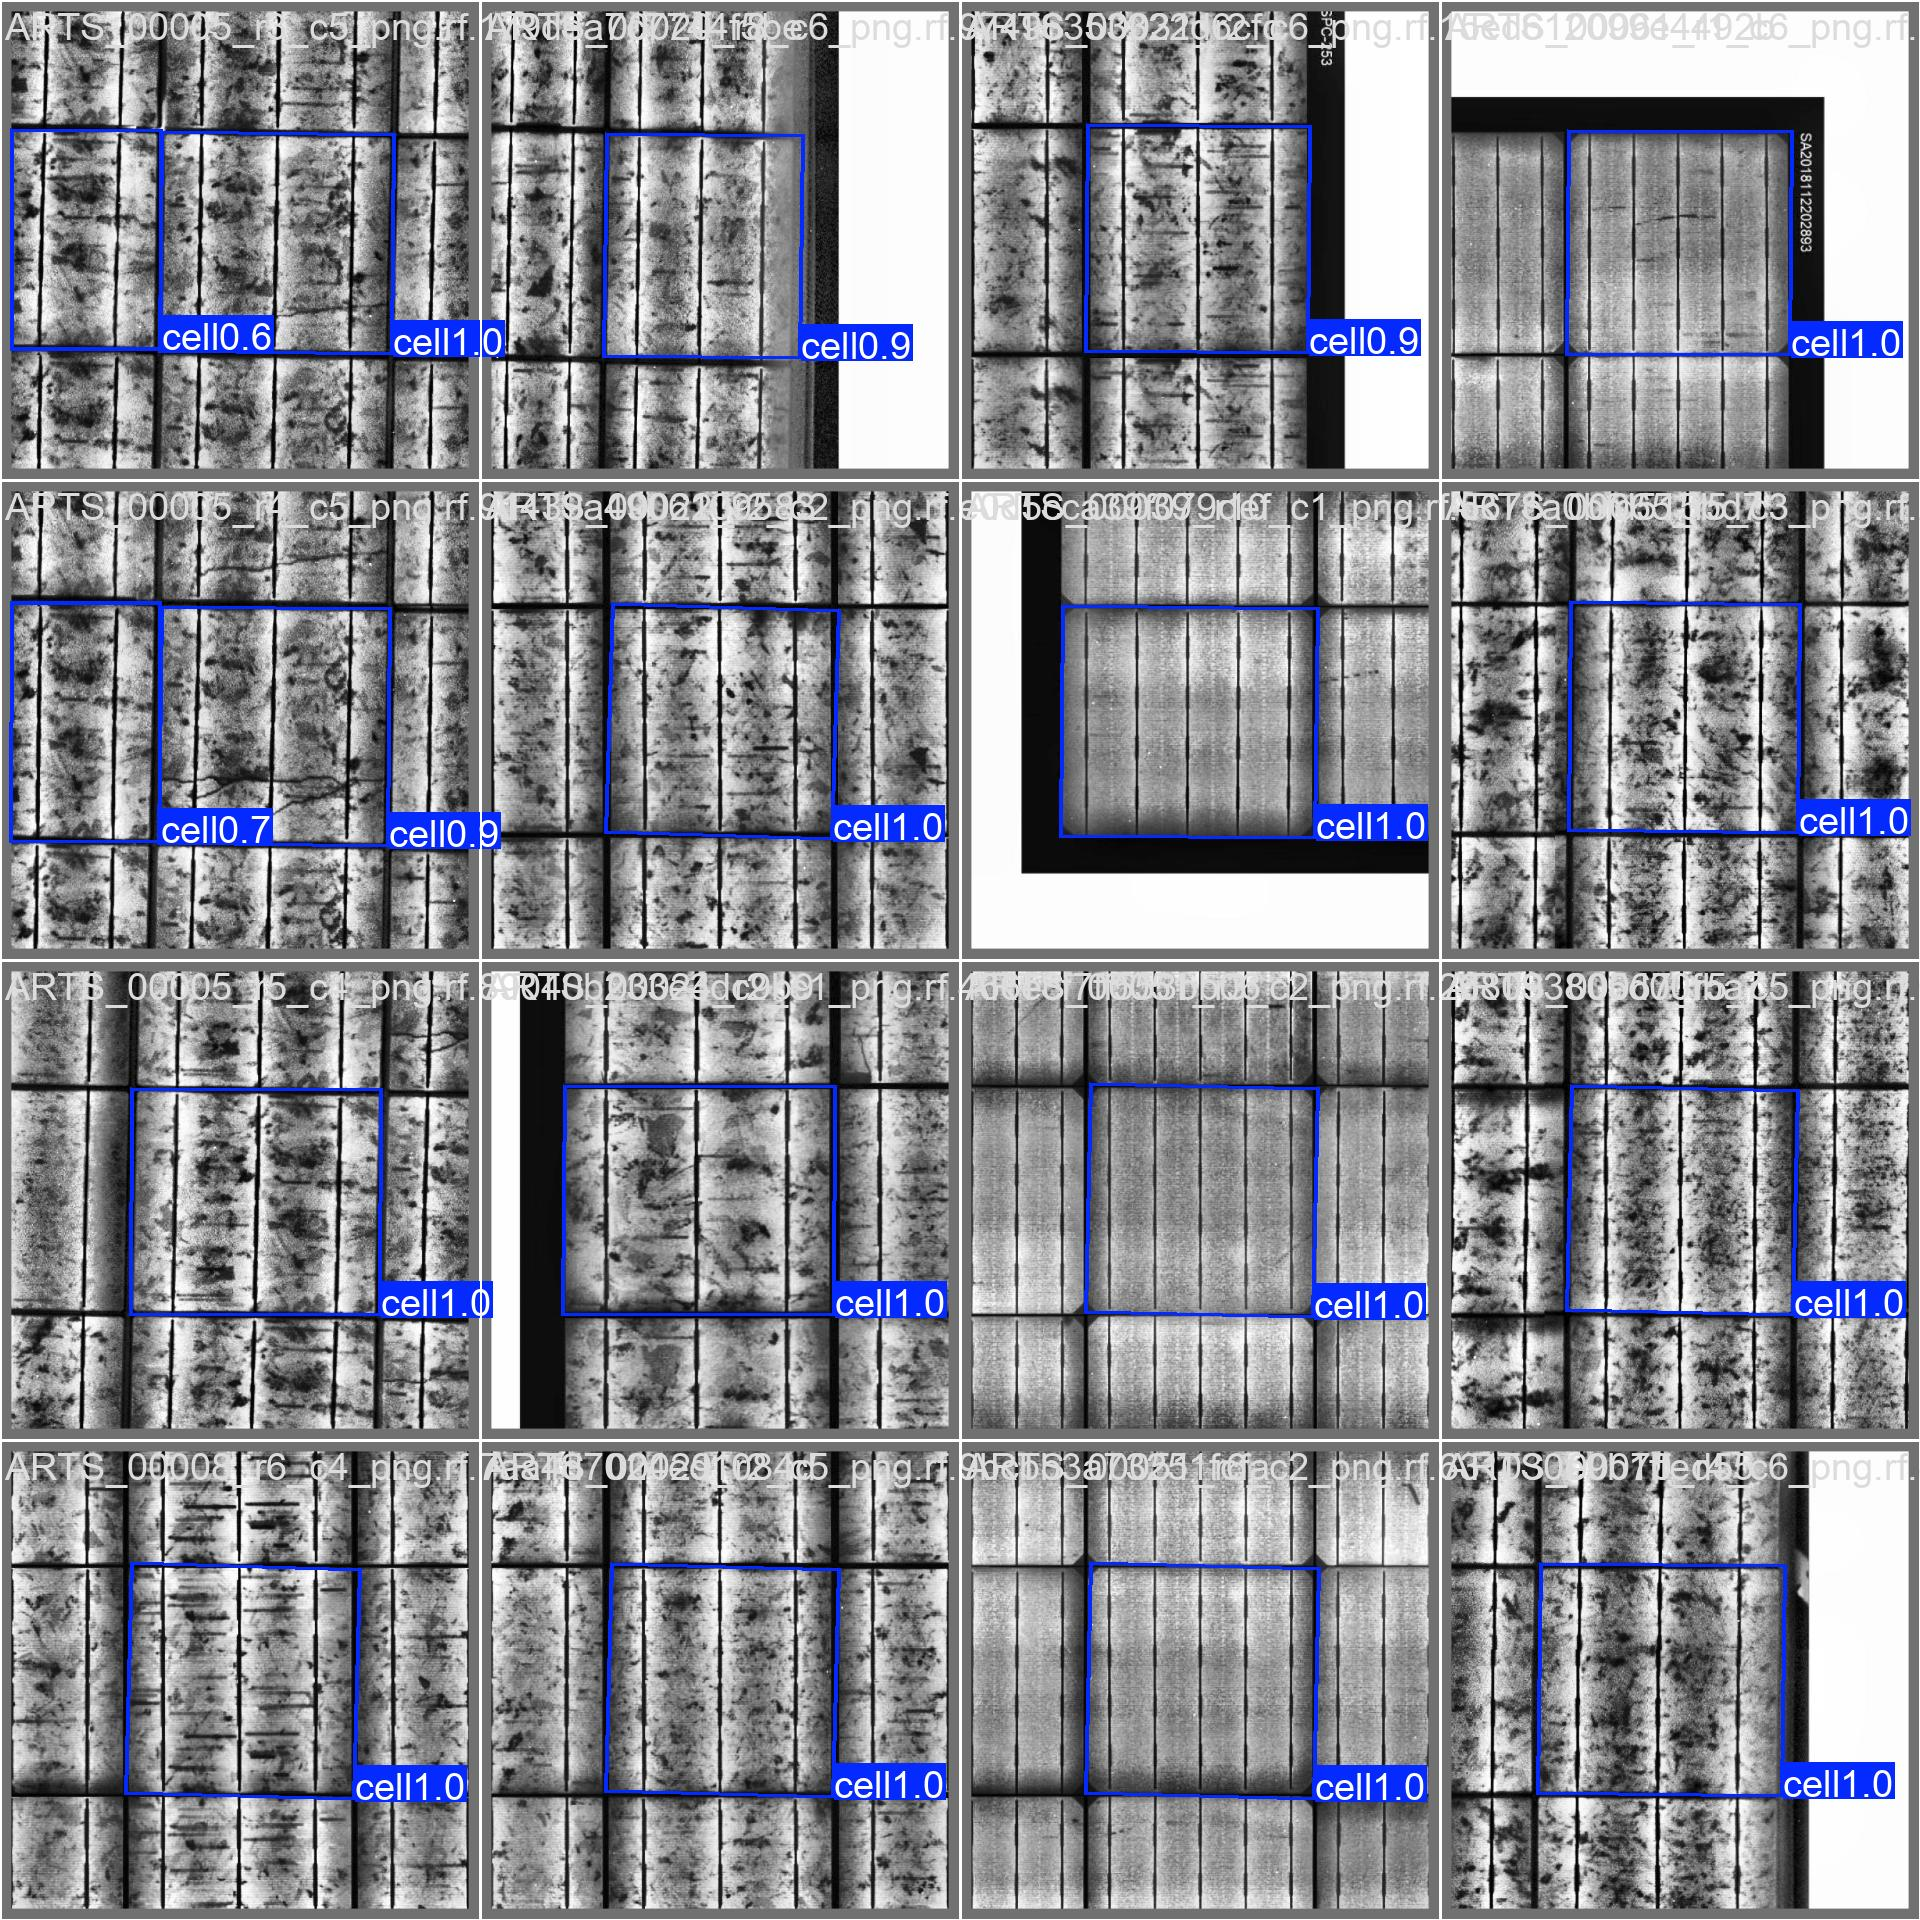
\includegraphics[width=\columnwidth,
        height=5.5cm,keepaspectratio=false]{fig_yolo_detections.jpg}}
  \caption{YOLOv8-OBB detections on a full-module EL image
           with oriented bounding boxes (top), and
           representative perspective-corrected cell crops
           (bottom). \textbf{[Replace with production figure.]}
           }
  \label{fig:yolo_detections}
\end{figure}

\subsection{Stage 2 --- Binary Quality Triage}
\label{sec:stage2}

\subsubsection{Architecture}

Each rectified cell crop $\hat{I}_{\text{cell}}$ is
classified as OK or B-grade by a pretrained CNN backbone
augmented with a CBAM block~\cite{woo2018} inserted after
the final convolutional stage, followed by global average
pooling, a dropout-regularised FC layer, and a sigmoid output.

CBAM applies dual attention sequentially.
\textit{Channel attention} selects defect-relevant feature maps:
\begin{equation}
  \mathbf{M}_c(\mathbf{F}) = \sigma\!\left(
    W_1\!\left(\text{ReLU}\!\left(W_0\,\text{GAP}(\mathbf{F})\right)\right) +
    W_1\!\left(\text{ReLU}\!\left(W_0\,\text{GMP}(\mathbf{F})\right)\right)
  \right)
  \label{eq:cbam_ch}
\end{equation}
\textit{Spatial attention} then suppresses background regions:
\begin{equation}
  \mathbf{M}_s(\mathbf{F}') = \sigma\!\left(
    f^{7\times7}\!\!\left(
      \left[\text{AvgPool}(\mathbf{F}');\,\text{MaxPool}(\mathbf{F}')\right]
    \right)\right)
  \label{eq:cbam_sp}
\end{equation}
where $\sigma$ is sigmoid, $W_0, W_1$ are MLP weights with
reduction ratio~$r$, $f^{7\times7}$ is a $7{\times}7$
convolution, and $\mathbf{F}' = \mathbf{M}_c \otimes \mathbf{F}$.
EL defect features occupy typically $<$5\,\% of cell area,
making CBAM's dual attention particularly effective without
localisation annotations.

\begin{figure}[t]
  \centering
  % PLACEHOLDER: Replace with Stage 2 CBAM architecture diagram
  \fbox{\parbox{\columnwidth}{\centering\vspace{1.8cm}
  \textbf{[PLACEHOLDER: Stage~2 CBAM Architecture Diagram]}\\
  Channel attention + Spatial attention modules,\\
  feature map shapes annotated.
  \vspace{1.8cm}}}
  \caption{CBAM dual-attention module inserted after the
           CNN backbone's final convolutional stage.
           \textbf{[Replace with production figure.]}
           }
  \label{fig:cbam_arch}
\end{figure}

\subsubsection{Hyperparameter Optimisation via Optuna}

Table~\ref{tab:optuna} lists the Optuna search space.
The optimisation objective is validation AUROC, chosen for
threshold-invariance under class imbalance.

\begin{table}[t]
  \caption{Optuna search space (Stage~2)}
  \label{tab:optuna}
  \begin{center}
  \renewcommand{\arraystretch}{1.05}
  \small
  \begin{tabular}{p{2.4cm}p{4.8cm}}
    \toprule
    \textbf{Hyperparameter} & \textbf{Search Space} \\
    \midrule
    Learning rate & LogUniform$[10^{-5},\;10^{-2}]$ \\
    Backbone & \{ResNet-18, ResNet-50, EffNet-B0, B3\} \\
    CBAM ratio $r$ & \{4, 8, 16\} \\
    Dropout rate & Uniform$[0.1,\;0.5]$ \\
    Batch size & \{16, 32, 64\} \\
    Optimizer & \{Adam, AdamW, SGD+momentum\} \\
    Objective & Validation AUROC \\
    \bottomrule
  \end{tabular}
  \end{center}
\end{table}

% ================================================================
%  SECTION V --- EXPERIMENTAL SETUP
% ================================================================
\section{Experimental Setup}
\label{sec:setup}

\textbf{Hardware:} \textbf{[TBD: GPU model, VRAM]}.

\textbf{Software:} Python~3.x, PyTorch~\textbf{[TBD]},
Ultralytics~8.3.235, \texttt{timm}~\textbf{[TBD]},
Optuna~\textbf{[TBD]}, OpenCV~4.12.0.88, NumPy~1.26.4,
scikit-learn~\textbf{[TBD]}, Matplotlib~3.8.4.

\textbf{Reproducibility:} All experiments run with $\geq$3
random seeds; results reported as mean\,$\pm$\,std.
Data splits are fixed prior to any training.

% ================================================================
%  SECTION VI --- RESULTS
% ================================================================
\section{Results}
\label{sec:results}

\subsection{Stage 1: Cell Extraction}

Table~\ref{tab:stage1_results} reports YOLOv8-OBB benchmark
results across five model scales on the test set.
All variants achieve mAP@0.5\,=\,0.995 with near-perfect
recall (1.0), confirming that the extraction task is solved
by data-driven OBB detection. The nano variant (YOLOv8n-OBB)
delivers 222~FPS at only 3.1M parameters, making it the
recommended deployment variant. The classical best
(FullModuleOpenCV fmv4) is included for reference; it requires
manual count verification per module and provides no
perspective correction.

\begin{table}[t]
  \caption{Stage~1 YOLOv8-OBB benchmark (test set)}
  \label{tab:stage1_results}
  \begin{center}
  \renewcommand{\arraystretch}{1.05}
  \small
  \begin{tabular}{lrrrr}
    \toprule
    \textbf{Model} &
    \textbf{Params} &
    \textbf{FPS} &
    \textbf{mAP@.5} &
    \textbf{mAP@.5:.95} \\
    \midrule
    YOLOv8n-OBB & 3.1M & \textbf{222} & 0.995 & 0.991 \\
    YOLOv8s-OBB & 11.4M & 216 & 0.995 & 0.993 \\
    YOLOv8m-OBB & 26.4M & 148 & 0.995 & 0.995 \\
    YOLOv8l-OBB & 44.5M & 118 & 0.995 & 0.992 \\
    YOLOv8x-OBB & 69.5M & 86  & 0.995 & 0.992 \\
    \midrule
    Classical (fmv4) & --- & --- & N/A & N/A \\
    \bottomrule
    \multicolumn{5}{l}{\footnotesize Classical: $\sim$90\,\%
    completeness (est.); no persp.\ correction.}
  \end{tabular}
  \end{center}
\end{table}

Fig.~\ref{fig:stage1_bench} shows the test mAP@0.5 comparison
across model scales.

\begin{figure}[t]
  \centering
  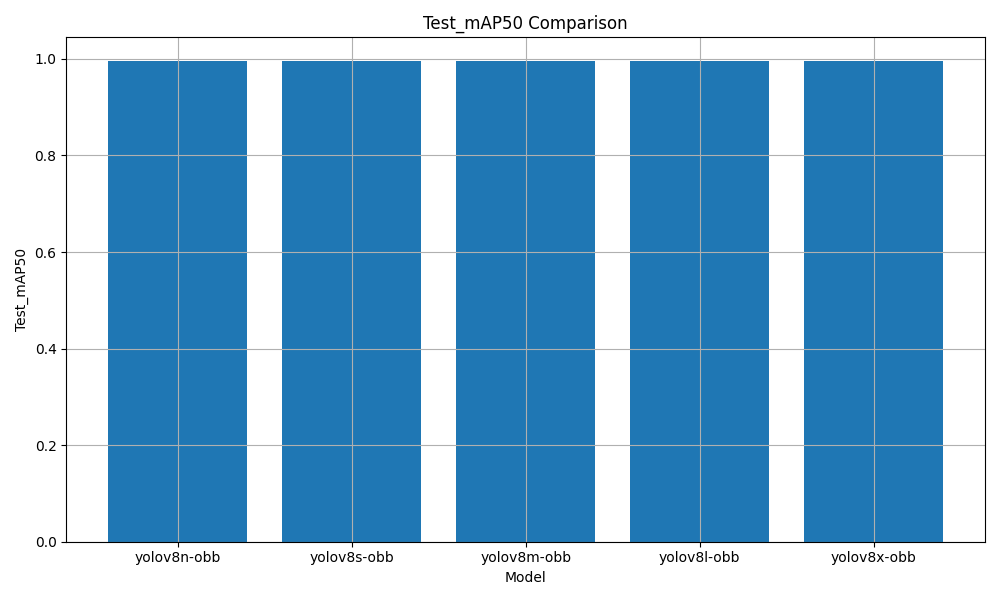
\includegraphics[width=\columnwidth]{fig_stage1_benchmark.png}
  \caption{YOLOv8-OBB model-scale comparison on test set
           mAP@0.5. All variants reach 0.995, confirming that
           even the lightest model saturates this task.}
  \label{fig:stage1_bench}
\end{figure}

\subsection{Stage 2: Binary Quality Triage}

Table~\ref{tab:stage2_results} shows the backbone and CBAM
ablation. CBAM contribution is isolated from Optuna tuning
by comparing rows~1--2 (same backbone, same LR, CBAM toggled).

\begin{table}[t]
  \caption{Stage~2 binary triage ablation results}
  \label{tab:stage2_results}
  \begin{center}
  \renewcommand{\arraystretch}{1.05}
  \small
  \begin{tabular}{p{1.8cm}ccp{0.8cm}p{0.6cm}p{1.1cm}}
    \toprule
    \textbf{Backbone} & \textbf{CBAM} &
    \textbf{Optuna} & \textbf{Acc.} &
    \textbf{F1} & \textbf{AUROC} \\
    \midrule
    ResNet-18  & No  & No  & [TBD] & [TBD] & [TBD] \\
    ResNet-18  & Yes & No  & [TBD] & [TBD] & [TBD] \\
    ResNet-50  & Yes & Yes & [TBD] & [TBD] & [TBD] \\
    EffNet-B0  & Yes & Yes & [TBD] & [TBD] & [TBD] \\
    EffNet-B3  & Yes & Yes & [TBD] & [TBD] & [TBD] \\
    \bottomrule
  \end{tabular}
  \end{center}
\end{table}

Results will be reported separately for monocrystalline and
polycrystalline cells. A placeholder for the Optuna trial
history figure (AUROC vs. trial number) is shown in
Fig.~\ref{fig:optuna_placeholder}.

\begin{figure}[t]
  \centering
  % PLACEHOLDER: Replace with actual Optuna trial history plot
  \fbox{\parbox{\columnwidth}{\centering\vspace{1.5cm}
  \textbf{[PLACEHOLDER: Optuna Trial History]}\\
  Validation AUROC vs. trial number.\\
  To be generated after Stage~2 experiments complete.
  \vspace{1.5cm}}}
  \caption{Optuna hyperparameter search convergence for
           Stage~2 (Validation AUROC vs.\ trial number).
           \textbf{[Replace with production figure.]}
           }
  \label{fig:optuna_placeholder}
\end{figure}

% ================================================================
%  SECTION VII --- DISCUSSION
% ================================================================
\section{Discussion}
\label{sec:discussion}

\subsection{Why Classical OpenCV Failed at Deployment Scale}

The 15-notebook exploration reveals four root causes.
\textit{Hyperparameter brittleness} manifests at every step:
CLAHE clip limits, Hough thresholds, and DBSCAN~$\epsilon$
tuned for one image break on the next due to natural EL
emission variation.
\textit{Module format sensitivity} is illustrated by fmv3,
where the projection-peak detector produced 208 cells (9
horizontal lines) for one module and 182 cells (8 horizontal
lines) for another nominally identical module.
\textit{Contrast variability} from degradation causes busbar
lines in low-EL regions to fall below adaptive threshold
limits.
\textit{Perspective intolerance} means even 5--10$^\circ$
tilt yields systematic misdetection in morphological
approaches.
YOLOv8-OBB subsumes all four into learned weights, at the
cost of requiring labelled training data.

\subsection{OBB Nano vs.\ Larger Scales}

Table~\ref{tab:stage1_results} demonstrates that mAP@0.5
saturates at 0.995 from YOLOv8n-OBB onward. The marginal
mAP@0.5:0.95 gain from nano (0.991) to medium (0.995) is
modest, while inference throughput drops from 222 to
148~FPS. For manufacturing-line deployment, YOLOv8n-OBB
is the recommended variant; for post-processing pipelines
where latency is not critical, YOLOv8m-OBB provides the
best precision-efficiency balance.

\subsection{CBAM for Spatially Localised Defect Features}

EL defects are spatially sparse ($<$5\,\% of cell area)
and spectrally discriminative---dark regions on a brighter
background. CBAM's channel attention selects defect-relevant
feature maps while spatial attention suppresses the uniform
background; together they are expected to yield measurable
F1 and AUROC gains (Table~\ref{tab:stage2_results},
rows~1 vs.\ 2) without requiring localisation annotations.

\subsection{Limitations}

\begin{itemize}
  \item \textit{Domain gap}: training data are lab EL images;
        field-collected EL introduces compression artefacts,
        variable exposure, and ambient light.
  \item \textit{Severity absent}: the pipeline produces a
        binary label but no continuous severity score.
  \item \textit{Annotation cost}: OBB labelling of 2{,}212
        full-module images is labour-intensive; semi-supervised
        strategies are a natural follow-on.
\end{itemize}

% ================================================================
%  SECTION VIII --- CONCLUSION AND FUTURE WORK
% ================================================================
\section{Conclusion and Future Work}
\label{sec:conclusion}

We have presented a two-stage automated inspection pipeline
for PV modules operating on raw module-level EL imagery.
A systematic ablation of 15 classical OpenCV approaches
establishes that grid-line detection cannot generalise across
deployment-scale diversity, motivating YOLOv8-OBB as a unified
Stage~1 cell extractor.
All five YOLOv8-OBB variants achieve mAP@0.5\,=\,0.995
on the test set, with the nano variant operating at 222~FPS.
Stage~2 binary triage with CBAM-augmented CNNs and
Optuna-based search addresses the coarse-label limitation
without localisation supervision.

\textbf{Future work} includes:
(1)~\textit{Stage~3 pixel-level defect segmentation} on
B-grade cells, consolidating 29 defect subtypes into four
physically motivated superclasses (crack, inactive area,
corrosion/metallisation, material/surface) and benchmarking
U-Net family against SegFormer~\cite{xie2021} with
Dice+Focal loss;
(2)~severity scoring calibrated against IV-curve power-loss
measurements;
(3)~instance-level defect localisation (Mask~R-CNN /
YOLOv11-Seg) for counting and spatial clustering;
(4)~domain adaptation from lab to field-acquired EL/IR
imagery; and
(5)~embedded GPU benchmarking (NVIDIA Jetson Orin) for
real-time manufacturing integration.

% ================================================================
%  ACKNOWLEDGMENT
% ================================================================
\section*{Acknowledgment}

This work was supported by the Indian Institute of Technology
Mandi. The authors thank their research supervisor for
invaluable guidance and support.

% ================================================================
%  REFERENCES
% ================================================================
\bibliographystyle{IEEEtran}
\bibliography{references}

\end{document}
